\documentclass[14pt]{beamer}
\usepackage[T2A]{fontenc}
\usepackage[utf8]{inputenc}
\usepackage[english,russian]{babel}
\usepackage{amssymb,amsfonts,amsmath,mathtext}
\usepackage{cite,enumerate,float,indentfirst}

\graphicspath{{images/}}

\usetheme{Pittsburgh}
\usecolortheme{whale}

\setbeamercolor{footline}{fg=blue}
\setbeamertemplate{footline}{
  \leavevmode%
  \hbox{%
  \begin{beamercolorbox}[wd=.333333\paperwidth,ht=2.25ex,dp=1ex,center]{}%
    Софийски университет
  \end{beamercolorbox}%
  \begin{beamercolorbox}[wd=.333333\paperwidth,ht=2.25ex,dp=1ex,center]{}%
    София, 2016
  \end{beamercolorbox}%
  \begin{beamercolorbox}[wd=.333333\paperwidth,ht=2.25ex,dp=1ex,right]{}%
  Стр. \insertframenumber{} из \inserttotalframenumber \hspace*{2ex}
  \end{beamercolorbox}}%
  \vskip0pt%
}

\newcommand{\itemi}{\item[\checkmark]}

\title{\small{Математически епидемиологически модели}}
\author{\small{%
\emph{Христо Вригазов}~\\%
\emph{Илия Жечев}~\\%
\emph{Виктор Божилов}~}\\%
\vspace{30pt}%
Приложение на математиката\\
за моделиране на реалните процеси%
\vspace{20pt}%
}
\date{\small{София, 2016}}

\begin{document}

\maketitle

\begin{frame}
\frametitle{Теми}
\begin{itemize}
  \item \textbf{SIR модел}
  \item \textbf{Метод на Ойлер}
  \item \textbf{Модел с клетъчен автомат}
\end{itemize}
\end{frame}

\begin{frame}
\frametitle{SIR модел}
\begin{itemize}
  \item Susceptible
  \item Infected
  \item Recovered
\end{itemize}
$$
\left\{
  \begin{array}{rl}
    S' = & - \beta SI \\
    I' = & \beta SI - \alpha I \\
    R' = & \alpha I
  \end{array}
\right.
$$
\end{frame}

\begin{frame}
\frametitle{Метод на Ойлер}
    \begin{figure}[H]
      \center
      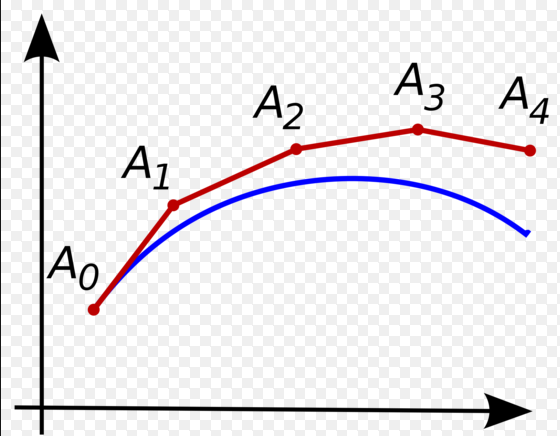
\includegraphics[width=0.8\linewidth]{Euler}
    \end{figure}
\end{frame}

\begin{frame}
\frametitle{Симулация на Python}
    \begin{figure}[H]
      \center
      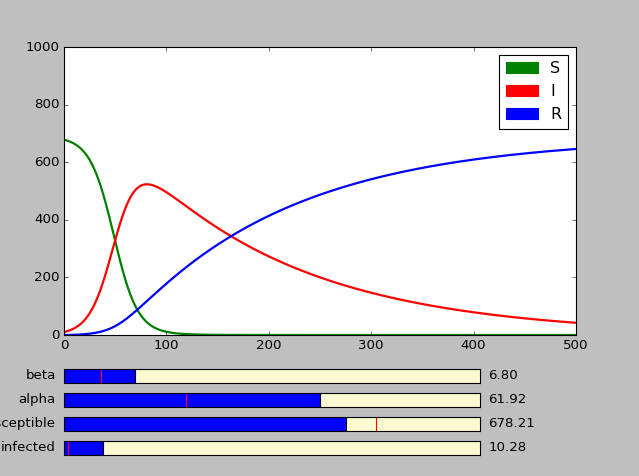
\includegraphics[width=0.8\linewidth]{python}
    \end{figure}
\end{frame}

\begin{frame}
\frametitle{Симулация с клетъчен автомат}
\begin{figure}[H]
  \center
  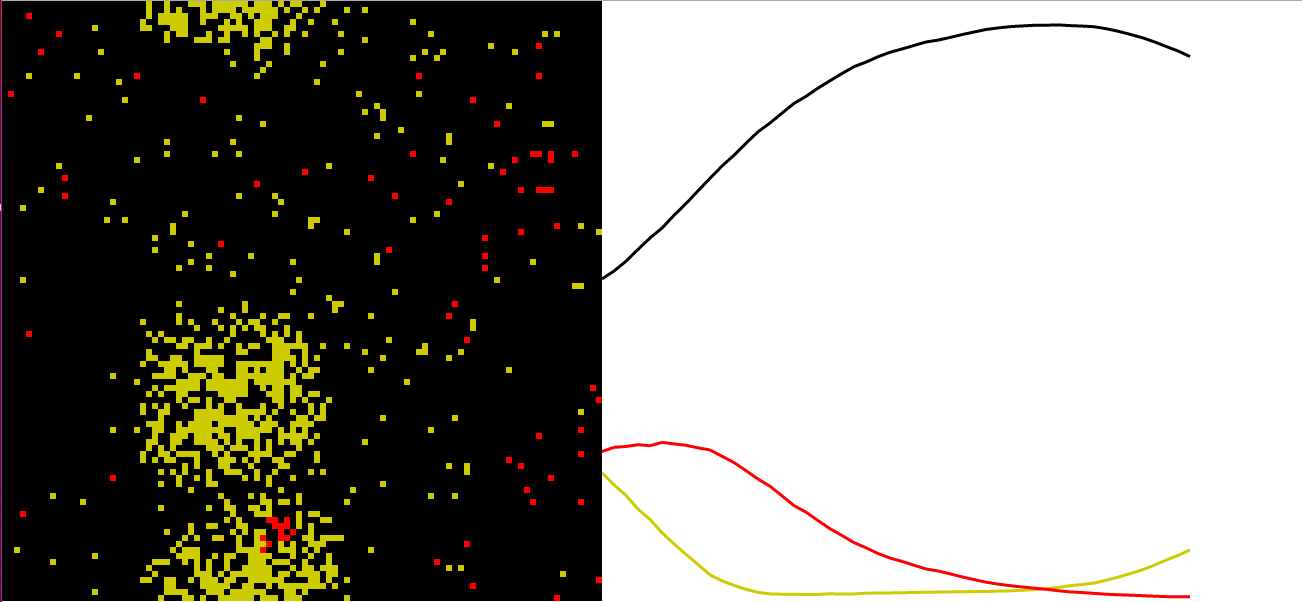
\includegraphics[width=0.8\linewidth]{automat}
\end{figure}
\end{frame}

\begin{frame}
\frametitle{Симулация с клетъчен автомат}
\begin{figure}[H]
  \center
  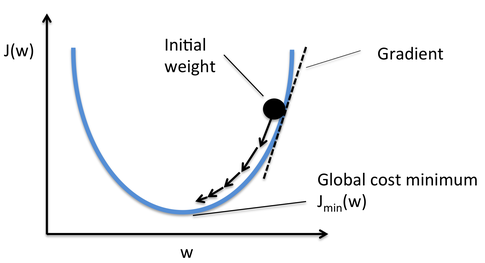
\includegraphics[width=0.8\linewidth]{gradient}
\end{figure}
\end{frame}



\begin{frame}
\begin{center}
Благодаря Ви за вниманието
\end{center}
\end{frame}

\end{document} 
